\documentclass{sig-alternate}
\usepackage[numbers, sort, compress]{natbib}
\usepackage{graphics}
\usepackage{graphicx}
\usepackage{epstopdf}
\usepackage{color}
\usepackage{hyperref}
\usepackage{pdfsync}
\usepackage{mdwlist}


\begin{document}

\conferenceinfo{TeraGrid 11} {}
\CopyrightYear{2011}
\crdata{}
%\clubpenalty=10000
%\widowpenalty = 10000


\title{Building Gateways for Life-Science Applications using the
  Distributed Adaptive Runtime Environment (DARE) Framework}

\numberofauthors{3}
\author{
\alignauthor Joohyun Kim\\
       \affaddr{Center for Computation and Technology}\\
       \affaddr{Louisiana State University}\\
       \affaddr{216 Johnston}\\
       \affaddr{Baton Rouge, LA} \\
       \email{jhkim@cct.lsu.edu}
\alignauthor Sharath Maddineni\\
       \affaddr{Center for Computation and Technology}\\
       \affaddr{Louisiana State University}\\
       \affaddr{216 Johnston}\\
       \affaddr{Baton Rouge, LA}
       \email{smaddineni@cct.lsu.edu}
\alignauthor Shantenu Jha\titlenote{Author for correspondence}\\
      \affaddr{Center for Computation and Technology}\\
     \affaddr{Louisiana State University}\\
      \affaddr{214 Johnston}\\
      \affaddr{Baton Rouge, LA}
     \email{sjha@cct.lsu.edu}
}

\maketitle


  % An understanding of challenges and computational requirements of
  % the life-science applications suggests that the uptake of
  % distributed heterogeneous scalable HPC resources demonstrate its
  % effectiveness as an integral component of a wide-range of
  % life-science gateways.  DARE science gateways comprise a user
  % access layer and middleware layers built upon Simple API for Grid
  % Application (SAGA) and the SAGA-based Pilot-Job (SAGA-BigJob)
  % capability.

\begin{abstract}
  This work is predicated on three important trends: (i) that the
  importance, impact and percentage of TeraGrid/XD resources assigned
  to the life sciences is increasing at a rate that is probably
  greater than other disciplines, (ii) that gateways have proven to be
  a very effective access mechanism to distributed HPC resources
  provided by the TG/XD, and in particular a very successful model for
  shared/community access models, and (iii) that there are missing
  capabilities and abstractions to enable the use of the collective
  capacity of distributed cyberinfrastructure such as TG/XD,
  especially those that can be used to develop gateways in an easy,
  extensible and scalable fashion for both compute-intensive and
  data-intensive applications.  We introduce the Distributed Adaptive
  Runtime Environment (DARE) framework that is a SAGA-based
  higher-level abstraction, and from which extensible, versatile
  gateway that seamlessly utilizes scalable infrastructure can be
  built for a life-science application effectively.  We discuss the
  architecture of DARE-framework based gateways, and four specific
  life-science gateways -- DARE-RFOLD, DARE-DOCK, DARE-HTHP and
  DARE-NGS, that use the DARE-framework to impart a wide-range of
  life-science capabilties.
\end{abstract}


% that allow a user to carry out RNA secondary structure prediction,
% virtual screening using a docking method, large-scale ensemble-based
% molecular dynamics simulations and alignment (mapping) of
% Next-Generation DNA sequencing data on a reference genome
% respectively.


%  We introduce the Distributed Adaptive Runtime Environment (DARE)
%   framework that is a SAGA-based higher-level abstraction, and
%   demonstrate its effectiveness as an integral component of a
%   wide-range of life-science gateways.  An understanding of challenges
%   and computational requirements of the life-science applications in
%   distributed heterogeneous scalable HPC resources has led to the
%   development of the DARE framework with which a lightweight,
%   extensible, versatile gateway that seamlessly utilizes scalable
%   infrastructure can be built for a life-science application
%   effectively.  DARE science gateways comprise a user access layer and
%   middleware layers built upon Simple API for Grid Application (SAGA)
%   and the SAGA-based Pilot-Job (SAGA-BigJob) capability.  This work is
%   predicated on three important trends: (i) that the importance,
%   impact and percentage of TeraGrid/XD resources assigned to the life
%   sciences is increasing at a rate that is probably greater than other
%   disciplines, (ii) that gateways have proven to be a very effective
%   access mechanism to distributed HPC resources provided by the TG/XD,
%   and in particular a very successful model for shared/community
%   access models, and (iii) that there are missing capabilities and
%   abstractions to enable the use of the collective capacity of
%   distributed cyberinfrastructure such as TG/XD, especially those that
%   can be used to develop gateways in an easy, extensible and scalable
%   fashion for both compute-intensive and data-intensive applications.
%   We present the framework and four specific life-science gateways --
%   DARE-RFOLD, DARE-DOCK, DARE-HTHP and DARE-NGS, that allow a user to
%   carry out RNA secondary structure prediction, virtual screening
%   using a docking method, large-scale ensemble-based molecular
%   dynamics simulations and alignment (mapping) of Next-Generation DNA
%   sequencing data on a reference genome respectively.

\newif\ifdraft
\drafttrue                                                                                        \
\ifdraft
% \newcommand{\reviewer}[1]{ {\textcolor{blue}    { ***Reviewer:     #1 }}}
 \newcommand{\jkimnote}[1]{{\textcolor{green}   { ***Joohyun:   #1 }}}
 \newcommand{\jhanote}[1]{  {\textcolor{red}     { ***SJ: #1 }}}
  \newcommand{\smnote}[1]{  {\textcolor{red}     { ***Sharath: #1 }}}
 \newcommand{\todo}[1]{  {\textcolor{red}     { ***TODO: #1 }}}
 \newcommand{\fix}[1]{  {\textcolor{red}     { ***FIX: #1 }}}
 \newcommand{\reviewer}[1]{}
\else
 \newcommand{\reviewer}[1]{}
 \newcommand{\jkimnote}[1]{}
 \newcommand{\smnote}[1]{}
 \newcommand{\jhanote}[1]{}
 \newcommand{\todo}[1]{  {\textcolor{red}     { ***TODO: #1 }}}
 \newcommand{\fix}[1]{}                                                                              
 \fi



\category{D.1.3}{Software}{Concurrent Programming}{ Distributed programming/parallel programming} 
\category{J.3}{Computer Applications}{Bioinformatics}

  % We use DARE as the underlying component for four different
  % Gateways that use both TG/XD resources as well as LONI
  % The middleware, in particular, owing to the core features provided
  % by SAGA such as interoperability, distributed scale-out,
  % extensibility, adaptivity, and simplicity (IDEAS) and a pilot job
  % abstraction, SAGA-BigJob,; facilitates a gateway developer to
  % implement a various execution patterns as well as distributed data
  % management.  By employing the DARE framework as well as the
  % SAGA/SAGA-BigJob, science gateways is able to provide a target
  % scientific application whose capacity is immediately enhanced with
  % distributed scalable HPC resources such as Teragrid and other
  % emerging computing environments such as clouds, consequently
  % advancing scientific computing, for example, by providing suitable
  % solutions for challenges in data-intensive scalable computing.

% A category with the (minimum) three required fields
%\category{H.4}{Information Systems Applications}{Miscellaneous} %Acategory including the fourth, optional field follows...
%\category{D.2.8}{Software Engineering}{Metrics}[complexity measures,performance measures]

\section*{General Terms}{Design,Measurement,Theory}

 \keywords{Science Gateway, Runtime Environment, Distributed Computing, Simple API for Grid
  Applications (SAGA), Pilot-Job abstraction, Data-intensive Computing}

% \keywords{ACM proceedings, \LaTeX, text
%   tagging} % NOT required for Proceedings
% \keywords{RNA conformation energy landscape, Runtime Environment,
%   SAM-I riboswitch, S gene of Bovine Corona Viral
%   Genome} % NOT required for Proceedings

%   It is interesting to note: (i) Molecular Biosciences represented
%   25\% of TeraGrid (NU) cycles used in Q1-2011.  (ii) Based on gateway
%   usage in first quarter of 20011, 3-4 of $\approx$ 20 TeraGrid
%   gateways currently are biogical/life science, which in turn account
%   for about $\approx$ 35\% of all gateway usage. (iii) However these 4
%   gateways account for about 2-3\% of recording molecular bioscience
%   usage. Points (i) - (iii) clearly imply that although a significant
%   fraction of TeraGrid cycles are devoted to Molecular Biosciences (of
%   which Molecular Dynamics is the dominant component), very few of the
%   MD users actually use gateways to access TeraGrid resources.  Given
%   the overall success and uptake of the gateways approach, prima
%   facie, there are reasons to belive that if a scalable, effective and
%   extensible capability were provided this {\it gap} could be
%   overcome. This provides an important motivation for the DARE-based
%   Science Gateways; 



\section{INTRODUCTION}

%\subsection{TeraGrid Usage by the life-science community}

The importance of computing in the life sciences has been well
appreciated. % An interesting corollary is that the rate-of-increase of
% computing resources devoted to the life sciences is increasing, and
% arguably is increasing at a rate faster than any other discipline.
In spite of fundamental limitations on the accuracy of the data, as
seen from Figs.~\ref{tg2007} \& \ref{tg2008} and Table~\ref{tg2011},
the trends are somewhat unambiguous: the percentage of TeraGrid
resources devoted to the life sciences is already more than any
discipline and the usage seems to be increasing on the back of other
disciplines, whether measured by number of cycles consumed, users or
allocations~\footnote{It is difficult to provide such information in a
  consistent way as the total number of cycles available year-to-year
  varies, but also which discipline a proposal gets assigned to is
  somewhat random; thus many chemistry proposals, even physics
  proposals are likely to be biological in nature}.

% The single largest community is the life-sciences community --
% including MD (25\%)...  Get a break-down of the total usage of the TG
% by discipline and application type.


\begin{figure}
 \centering
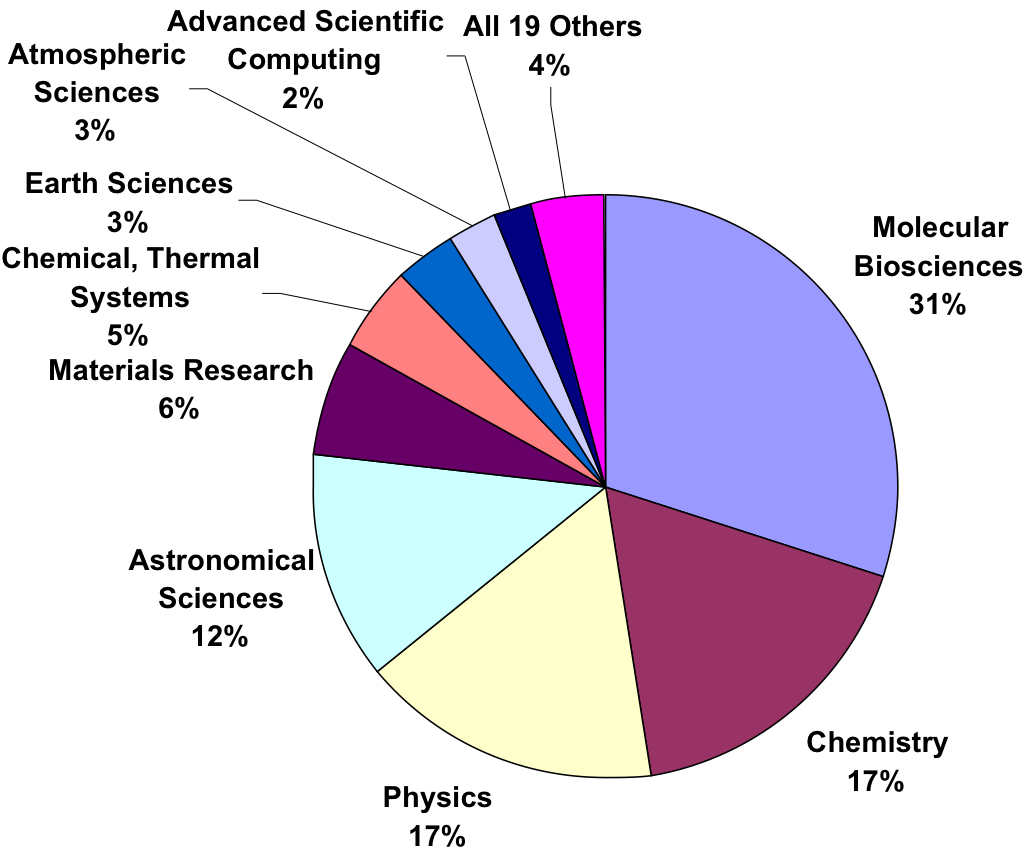
\includegraphics[scale=0.40]{figures/teragrid-discipline07}
\caption{\small 2007 Usage statistics for the TeraGrid.  (Reference
  \url{http://www.teragridforum.org/mediawiki/images/9/90/II_WorkShop_G-HPC_Nework_2009-Towns.pdf})}
  \label{tg2007}
\end{figure}


% \subsection{Large scale life-science applications on the distributed
%   HPC resources}
% Traditionally, life-science applications have been regarded as non-HPC
% applications.  Notably, only a few applications were actively pursued
% with large scale computations.  Two representative examples are
% molecular simulations and virtual docking calculations.
% Interestingly, while the former represents the case that the so-called
% scale up of bulk synchronous techniques such as MPI is used as a main
% strategy to deal with larger molecular systems, the latter represents
% the case that massive independent tasks should be carried out,
% representing two different application usage modes.


With the exception of a few applications, e.g., large-scale
simulations (mostly MD) and virtual-docking simulations, most
% science applications most
life-science applications have not been very effective in utilizing
HPC cyberinfrastructure.  Interestingly, MD simulations have mostly
relied on scaling-up to high core-counts; virtual docking has been
dependend on high-throughput.  However the need of large-scale
distributed parallel executions for other other areas of
biological/life-science applications is growing due to the advances of
experimental techniques employing high-throughput approaches as well
as the advent of computing power and data management capacity.  For
example, Next-Generation DNA Sequencing (hereafter, NGS) technologies
challenge computational biology with unprecedented amounts of data
produced by their high-throughput capability.  Required data analytics
for processing such sequenced data along with dealing with genome data
sets available in public and private databases are overwhelmed by the
pace of growing data volume.  This poses the question of how the
challenges with large volume data-management as well as the
computational requirements for analyzing large volumes of data are
effectively managed.


Interestingly, the cyberinfrastructure considerations required to
support a broad-range of analytical approaches and at the scales
required, has received less attention than the data-management problem
and algorithmic advances.  Thus not surprisingly, traditional
production cyberinfrastructure, such as the TeraGrid, have not been
used for such data-intensive analytics and distributed
applications. There are multiple reasons, but a couple of contributing
factors are: (i) insufficient runtime environments (and abstractions)
to support concurrent computational capabilities with large-data sets
to support data-analytics (beyond visualization) in an easy, scalable
and extensible fashion, (ii) insufficient support for
user-customizable data-intensive "workflows" that effectively hide the
challenges of data-movement and efficient data-management whilst
managing concurrent distributed (computational) resources.

% Indeed, molecular simulations, virtual screening, and many other
% bioinformatics applications, particularly, regarded as the non-HPC
% applications could increase their usages dramatically by utilizing
% distributed scalable resources, which is, as presented in this work,
% addressed by a gateway development that implements a runtime
% environment for executions of target computation and distributed data
% management.

It is interesting to note~\footnote{Based upon shared
  information/private commmunication between SJ and Dave Hart \& Dan
  Katz}: (i) Molecular Biosciences represented 25\% of TeraGrid (NU)
cycles used in Q1-2011.  (ii) Based on gateway usage in first quarter
of 20011, 3-4 of $\approx$ 20 TeraGrid gateways currently are
biogical/life science, which in turn account for about $\approx$ 35\%
of all gateway usage. (iii) However these 4 gateways account for about
2-3\% of recording molecular bioscience usage. Points (i) - (iii)
clearly imply that although a significant fraction of TeraGrid cycles
are devoted to Molecular Biosciences (of which Molecular Dynamics is
the dominant component), very few of the MD users actually use
gateways to access TeraGrid resources.  Given the overall success and
uptake of the gateways approach, prima facie, there are reasons to
belive that if a scalable, effective and extensible capability were
provided this {\it gap} could be overcome.
 

\begin{figure}
 \centering
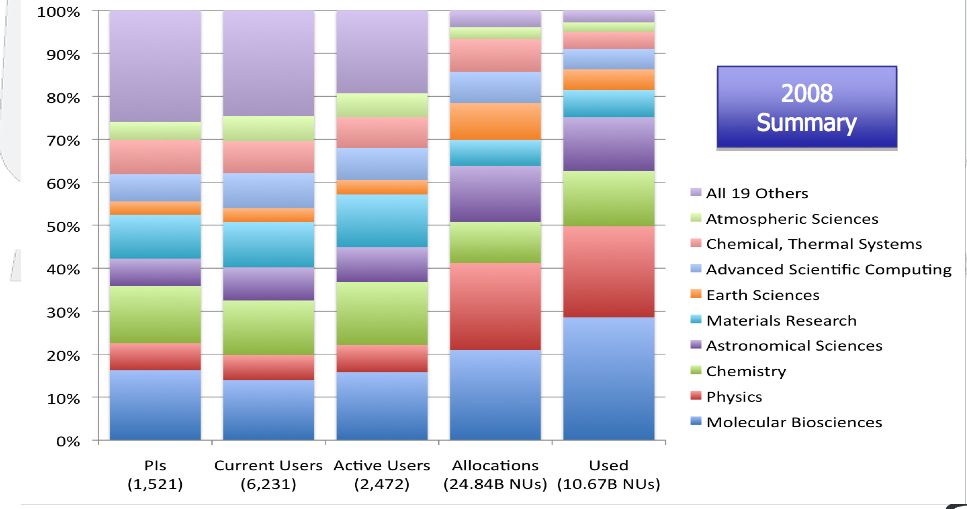
\includegraphics[scale=0.27]{figures/teragrid-discipline08}
\caption{\small 2008 Usage statistics for the TeraGrid (Reference
  \url{http://www.teragridforum.org/mediawiki/images/d/d8/DEISA-PRACE-May2009-Towns.pdf})}
  \label{tg2008}
\end{figure}

Additionally, TeraGrid Science gateways have witnessed
impressive achievements in terms of the growth of the number of
supporting researchers and computing time usages.  Those gateway developments are often helped by suites of tools such as the Open Grid Computing Environments\cite{ogce-2010}.  However, most of
gateways do not support distributed execution, i.e., most gateways
still enforce the tight-coupling between applications and specific
resources.  A primary reason is the additional, not insignificant
complexity to transform a target application to be able to seamlessly
utilized distributed cyberinfrastructure, and thus into a distributed
application.  In other words, it is non-trivial to meet the
developmental objectives for distributed applications, viz.,
interoperability, distributed scale-out, extensibility, adaptivity,
simplicity-taken together referred as IDEAS\cite{ideas}, mainly due to
the lack of tools for the coordination over multiple and distributed
compute/data sites.

We observe with the advent of federated grids such as Teragrid and its
transition to eXtreme Digital (XD) environment, such requirements
become harder to achieve as the number of connected sites grows as
well as the computing power and the data storage capacity of each
resource reach peta or exa scales.  More importantly, supporting a
broad range of diverse execution patterns is critical considering
different application usage modes for different life-science
applications.  For example, in Table~\ref{table:four-applications},
application usages for four life-science applications focused on this
work are summarized by contrasting conventional vs. distributed modes.
Last not the least, it is always challenging to respond effectively to
the upcoming demands of supporting new applications, distributed data
management with new infrastructure, implementation of novel execution
patterns, which is often eased by the development of a framework and
its use for the efficiency in development cycle.
 
\begin{table}
 \small
\begin{tabular}{|c|c|c|c|c|c|} 
  \hline  Quarter & PIs & Current & Active & Allocations  & Usage\\
  & & Users  &  Users & (NUs) $\times 10^6$& (NUs) $\times 10^6$ \\ \hline
  Q3 2010 & 249 & 1,044 & 366 & 8,810   & 2,219  \\ \hline
  Q4 2010 & 254 & 1,040 & 356 & 11,720  & 2,658, \\ \hline
  Q1 2011 & 257 & 1,168 & 418 & 13,101  & 3,412\\ \hline 
\end{tabular} 
\caption{Life-Science usage of the TeraGrid over the recent
  quarters. The figures establish that both the  allocation and the
  usage of life-science applications is increasing at least in
  proportion to the increasing resource availability on the TeraGrid,
  if not faster.}
 \label{tg2011} 
\end{table}

This work is predicated on three important trends: (i) that the
importance, impact and percentage of TeraGrid/XD resources assigned to
the life sciences is increasing at a rate that is probably greater
than other disciplines, (ii) that gateways have proven to be a very
effective access mechanism to distributed HPC resources provided by
the TG/XD (and in particular a very successful model for
shared/community access models); given the landscape of the future
distributed cyberinfrastructure, we anticipate the importance of
gateways will continue to increase, and (iii) that there are missing
capabilities and abstractions to enable the use of the collective
capacity of distributed cyberinfrastructure such as TG/XD, especially
those that can be used to develop gateways in an easy, extensible and
scalable fashion for both compute-intensive and data-intensive
applications.

As a modest step towards addressing point (iii), we have shown that a
flexible Pilot-Job framework can provide the ability to run multiple
MD simulations effectively across multiple resources on the
TeraGird~\cite{saga-royalsoc, saga-ccgrid10}. Specifically, we've
shown how a SAGA-based framework, such as the pilot-job framework
supports the distributed application design objectives categorised by
the term IDEAS -- Interoperable, Distributable (Scale-Out),
Extensible, Adaptive and Simple~\cite{ideas}.  In this paper we
establish how these capabilties can be generalized and provided via
gateways, to support a range of life-science applications.  We
introduce the SAGA-based DARE framework and establish its
effectiveness as an integral component for four different life-science
gateways by demonstrating that it can effectively utilize the
collective capabilities of distributed cyberinfrastructure such as the
TeraGrid/XD. We use DARE as the underlying component for four
different gateways that use both TG/XD resources as well as LONI
resources.

% \subsection{Challenges in developing a gateway supporting distributed
%   applications with heterogeneous multiple HPC resources}


\section{FOUR LIFE-SCIENCE APPLICATIONS}

\begin{table}
 \small
\begin{tabular}{|c|c|c|c|} 
  \hline Science  & Supported  & Conventional   &   Distributed
  \\
  Domain & Appli- & Application & Application \\ 
  &  cation(s) & Usage Mode & Usage Mode \\  \hline \hline 
  
  Molecular   &  \texttt{NAMD} &  MPI-based  & ensemble-based   \\
  Dynamics  &  & single simulation  & multiple  \\ 
  &  & run &  simulation  \\ 
  &  &  &  runs \\ \hline
  RNA   & \texttt{SFOLD}, & short single task    & large number  \\
  Folding   & \texttt{RNAFold} & or a few serial & of tasks using   \\
  Prediction & &  tasks &distributed \\
  &  &  &   resources  \\ \hline
  NGS data     &  \texttt{BFAST} & memory-intensive  & data-intensive\\ 
  analytics  &  &  single-node   &  distributed  \\
  & & exeuction  & computing \\ \hline
  Virtual  & \texttt{Autodock} &  many tasks   & many tasks \\
  Screening  &  & using a cluster  & using multiple  \\
  (Docking) &  &  & resources \\ \hline
  \hline
\end{tabular} \caption{Four life-science applications of interest and their usage modes.  Four gateways were developed for these applications using the DARE framework}
 \label{table:four-applications} 
\end{table}

Here we describe the four scientific applications briefly around the
aspects primarily focused by the gateway development using the DARE
framework

\textit{Large scale Molecular Dynamics simulations:} Over the past two
decades, the field of biomolecular simulation has exploded due to
increases in computational power and parallel codes, the emergence of
accurate molecular mechanical potentials or force fields and
improvements in the methods~\cite{amber,mackerell2008,adcock2006}. A
continually growing body of researchers apply atomistic and
coarse-grained molecular dynamics (MD) simulation methods to
facilitate drug discovery, perform advanced materials research, to
design and understand biomolecular and designed catalysts, and to
provide fundamental insight into molecular structure, dynamics and
interactions\cite{meinke2009,mcdowell2006,beck2007}.

%Particular challenges include de
%novo protein and nucleic acid folding and structure prediction;
%correctly modeling induced-fit and conformational selection as drugs
%or other molecules interact with a target macromolecule; modeling
%large ensembles of biomolecules such as proteins in a membrane
%environment, viruses, and biomolecular machines such as the ribosome;
%combined quantum and molecular mechanical treatments for modeling
%chemistry; and improving conformational sampling and estimation of
%free energies and free energy pathways. 

In response to the perceived needs and importance of molecular
simulations, numerous high performance distributed memory parallel
codes have emerged in the past two decades (including NAMD, CHARMM,
AMBER, LAMMPS,GROMACS, etc.), and many now can directly include
quantum representations.  An interesting challenge in the MD community
is, along with continuing efforts that tackle more scalable molecular
systems with longer time trajectories using more powerful machines, to
develop ensemble-based simulations over multiple HPC resources.

\textit{NGS-driven genome data analytics:} In the past several years,
there has been a major paradigm shift in biological/biomedical
researches with the Next-Generation DNA Sequencing
technologies\cite{mardis2008-tig,metzker2010,mardis2008-arghg}.  Their
novel capabilities of cost-effective resequencing, full-scale
quantitative transcriptomics, and holistic approach for cell
development and cell differentiation using protocols such as
RNA-seq. and ChIP-seq opens a completely new era for life-science
researches\cite{sorek2010,mortazavi2008}.  In spite of such great
opportunities, current NGS platforms challenges data analytics to deal
with the sequencing data and the following bioinformatics analysis and
inference.  For example, at this moment, NGS platforms produce
typically billions of reads that comprise a short sequence mostly less
than 100 base pairs with most of real experimental
setting\cite{alex2009,trapnell2009}.  Furthermore, the increasingly
effective cost-down trend causes the difficulty in management of
significant size of data produced or related data sets that should be
analyzed together.  Bioinformatics tools for NGS data analytics are
numerous and there is no sign to see the end of influx of new tools
considering continuous innovations in the technologies and algorithmic
advances in such tools, implying the simplicity and the extensibility
of an gateway development approach is important.  With the current
implementation, we focus on the most important analysis of NGS data,
mapping of NGS reads on a reference genome.  Soon, this analysis step
is extended to support a broad range of following analyses targeting
specific research goals such as genome variation, genome-wide
association, comparative genomics, and other applications for
investigating biological processes in a living cell.

\textit{RNA structure prediction and beyond:} Defying the old
biological dogma, positioning RNAs as a genome information
intermediate between DNAs and proteins, during the last couple of
decades, the number of scientific observations found that RNAs were
actively involved significantly in gene expression and
regulation\cite{joyce1999,cruz2009,encode2007,amaral2008}.  Now, with
the well-known categories of non-coding RNAs such as miRNAs and
riboswitches, in spite of their biogenesis that does not need to be
translated into proteins, significant roles of RNAs are quite well
recognized\cite{costa2009,ellington2007,baek2008,blouin2009,henkin2009}.
Importantly, RNA functions by forming required structure(s), and the
pattern of structure formation of RNAs are somewhat contrasted to
proteins that are mostly folded into highly specific 3-D
structure\cite{roth2009}. For example, riboswitches chose one of two
alternative structures, in response to metabolite binding,
consequently resulting in two different gene regulation stages, i.e.,
turning on downstream gene synthesis or turning it
off\cite{montange2008,dambach2009,weinberg2007}.  Therefore, RNA
structure prediction has been the major area for RNA studies and may
noticeable progresses were made recently for RNA 2D structure
prediction as well as 3D structure
modeling\cite{shapiro2007,mathews2006,ding2003}.

\textit{Drug Discovery via Virtual Screening strategies:} For small
molecule drug discovery, virtual screening using a docking method has
been widely utilized and an immediate requirement for massive docking
calculations against a chemical database has been attempted by
managing such many tasks using a local cluster, HPC cluster, grids,
and clouds\cite{levesque2009,yim2010}.  The nature of required
application usage mode for virtual screening methods is a generic
example of many task computing, implying that pleasingly parallel
massive tasks carrying out a docking computation should be executed.
In spite of such well-established protocol, the challenges in drug
discovery finding putative inhibitors for target receptors are not
resolved due to intrinsic difficulties with underlying
physico-chemical models associated with the issues with scoring
function, receptor flexibility, and docking strategy
itself\cite{amaro2010}.  Therefore, more computing power and scaled
calculations by varying the parameters for virtual screening are
needed in order to understand the accuracy of results, suggesting the
need of scalable infrastructure is highly appreciated while the
application usage mode is generally intact.

\subsection{Computational requirements and challenges}

A growing limitation of applications in the life sciences is that
workflow, data management, and analysis have become rate limiting
steps: what is missing is support for the end-to-end execution
requirement of applications.

We also need to move to tiered sets of computational resources.  For
example, one can imagine running large ensembles of MD engines on
tightly coupled parallel machines (like Ranger or Kraken) with
real-time data streamed to separately running analysis and
visualization resources (Lonestar, Spur), with on-the-fly monitoring
to analyze convergence, interesting phenomena or problems.  This also
provides the means for possible steering, for example by spawning or
stopping separate elements of the ensemble to sample more or less in a
particular region of interest.  In addition to real time monitoring,
hidden correlations in the data require the saving of coarser grained
simulation data on longer term (1-2 year) disk resources for further
analysis and mining using less tightly coupled computational
resources, and ultimately placing reduced and derived data sets
seamlessly back to the campuses, archivers, and for public
distribution.  Not only does this support the need for diverse sets of
computational resources, large-scale storage and data transfer
requirements for sophisticated analysis and visualization, and
high-bandwidth networking, it also drives the need for software tools
that facilitate the complicated workflow management, that allow
dynamic monitoring, starting and stopping of ensemble elements without
losing access to the global communications fabric and local
connections, and that provide the means for facilitating data
management and analysis.

In essence, the move from executing an individual task to
\textit{large ensembles} of coupled/loosely/uncoupled tasks requires
scientists to spend significant time on compute and data management
problems, instead of core science.  The quantitative shift (massive
distributed parallel compute and data resources) implies qualitative
change in the way how life-science applications are being served for
scientific discovery.


\section{DISTRIBUTED ADAPTIVE RUNTIME ENVIRONMENT}

We develop the Distributed Adaptive Runtime Environment (DARE)
framework\cite{dareurl}, in order to provide the means for the rapid
development of gateways that enable a scientific application to
utilize scalable heterogeneous distributed computing resources.

As shown in Fig.~\ref{fig:dare-arch}, an architecture of a gateway
based on the DARE-framework comprises of the classic three layers: (i)
the Access/Application Layer, (ii) the Services/Middleware Layer, and (iii) the
Resource, whose underlying development mechanisms are independent and
modular but unified under the framework.  The Access/Application layer
employs the open source web application framework,
pylons\cite{pylonsurl}.  The core/functional layer of this
architecture -- the Services/Middleware Layer is powered by SAGA and
SAGA-based Pilot-Job capabilt, the SAGA-BigJob\cite{saga-ccgrid10,jha2009developing,ecmls10, ecmls11},
collectively constituting a runtime environment for distributed
applications.

We will show how the combination of the open-source web application
technology, the runtime environment to support distributed execution
application enables the effective and quick construction of
lightweight, extensible, gateways that can effectively utilize
distributed cyberinfrastructure. But first we briefly describe
SAGA/SAGA-BigJob which forms a core component of the
Services/Middleware layer.

\subsection{SAGA and SAGA-BigJob abstraction}

SAGA is an API that provides the basic functionality for developing
distributed applications, tools and frameworks\cite{saga-web}. The key
advantages of the development using SAGA include, but are not limited
to: i) to provide a general-purpose, commonly used yet standardized
functionality, while hiding complexity of heterogeneity of back-end
resources, ii) to provide building blocks for constructing higher-level
functionality and abstractions iii) to provide the means for
developing broad range of distributed applications such as gateways,
workflows, application management systems, and runtime environments.
Interestingly, SAGA provides a simple way to support scripting
for building distributed applications via python-binding. 

SAGA-BigJob~\cite{saga-ccgrid10} was introduced as a general-purpose
pilot-job framework, with which various execution patterns and
application usage modes have been
supported~\cite{async_repex11,saga-royalsoc}.  Previously, we
demonstrated how SAGA-BigJob was able to execute scientific
applications categorized as pleasingly parallel applications and
loosely coupled applications in scalable distributed
resources\cite{jha2009developing, ecmls10, ecmls11}

As we will show in \S4, building the DARE framework on SAGA and
SAGA-BigJob, the fundamental design objectives of Interoperability
across different infrastructure, Distributed Scale-Out, Extensibility,
Adaptivity whilst preserving Simplicity (IDEAS)\cite{ideas}, which
constitutes essential requirement for distributed applications, are
achieved in a remarkably effective way.

\subsection{Three Layers Architecture of DARE-enabled Science
  Gateways}

% -- Access/Application Layer, Services/Middleware Layer, and Resource
% Layer}

\begin{figure}
  \centering
  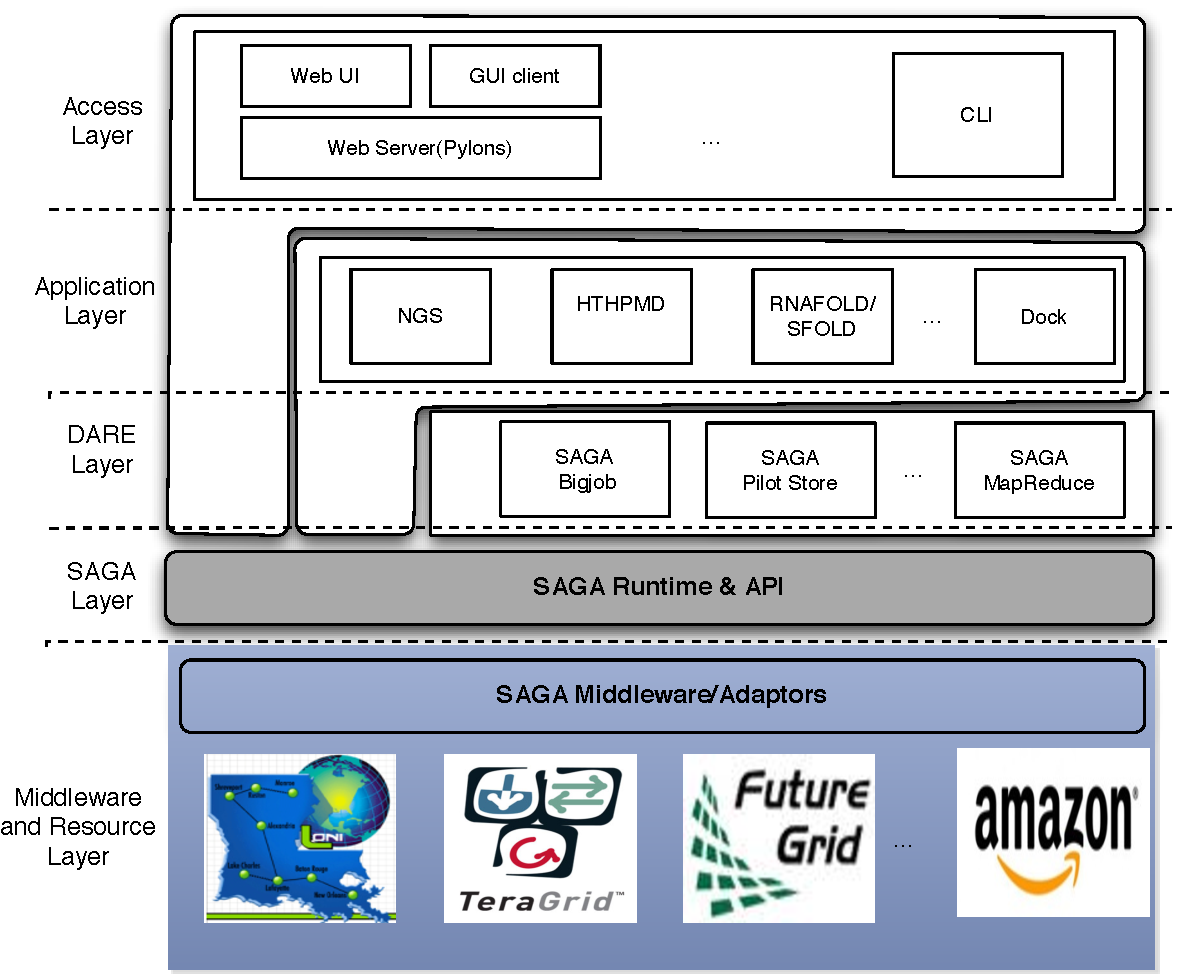
\includegraphics[scale=0.40]{figures/DAREOutline.pdf}
\caption{\small Architecture of DARE enabled science gateways }
  \label{fig:dare-arch} 
\end{figure}

\textit{Access/Application Layer:} The combination of the Access Layer
and the Application Layer is the only component a developer needs to
implement his/her own scientific logics and user interface (UI)
design.  The Access Layer is composed of a web server and UI.  UI
mediates the interactions between a user and a web server, and is
primarily important for enhancing user experience.  Depending upon
types of UI, three-tier or two-tier gateway structures are possible.
For example, if the web server is accessed via web pages or a remote
client, the overall architecture is regarded as a three-tier
architecture in which a user desktop, a server, and back-end resources
are independent to each other and their connection is under control by
the DARE framework.  Currently, the framework employs the use of web
UI as a primary means for a user access.  On the other hand, if
Command Line Interface (CLI) is preferred, the overall architecture
becomes two-tier since there exist no need of a system for a remote
user.

The Model-View-Controller (MVC) architecture model that underlies the
pylons web application framework is very effective and advantageous in
many ways. For example, database creation, management, and transaction
are extremely simple and robust to facilitate authentication steps and
job/data creation and management by storing or retrieving related
data.  Additionally, UI creation/development and the connection
between server-side services (provided by the Services Layer) and
UI-based user interactions are also surprisingly simpler compared to
other existing approaches, requiring less programming efforts.  For
example, it is well appreciated that for a science gateway
development, the utilization of databases and server-side programming
are non-trivial tasks.

The Application Layer is the core part for the gateway development,
since as target scientific applications differ in optimal application
usage modes along with favorable execution patterns implemented
differently with heterogeneous distributed resources, it is a
developer's responsibility to find a better science logics and
implementation, which is often non-trivial if distributed resources
and distributed data management are needed.  However, the underlying
Services and Middleware Layer mitigates such developmental hassles
owing to SAGA-based technology.

\textit{Services/Middleware Layer:} The challenges to build a scalable
distributed gateway is greatly facilitated by SAGA and SAGA-BigJob.
For example, by varying SAGA-BigJob configuration with a minimal
developmental effort, it is easily accomplished to optimize execution
usages of target computations at the same time properly considering
their application characteristics such as pleasingly parallel, loosely
coupled, or in a certain case, strongly coupled applications.  As
demonstrated in this work presenting four different gateways for four
different life-science applications, once figuring out preferable
application usage modes as well as parallelization strategies, a
gateway developer easily constructs an optimized runtime environment
for a target application with distributed resources in a relatively
short development cycle.

%The web interface will be connected to remote job submission via a job scheduling and monitoring thread. This thread starts with pylons application and continuously communicates with local database server to find new jobs and it also acts as a scheduler for new jobs. Once this thread finds a new jobs it will start preparing the configuration files for that particular job from the user and afterwords it will start the remote job submission via application specific SAGA-Bigjob.

Importantly, data movement should be carefully considered when a
gateway is developed, since the movement of large data sets such as
input, output, temporary files is increasingly becoming a major
challenge. We have shown recently analyzed the volumes that need to be
shipped, and demonstrated some of the challenges and solutions in the
case of a next-generation sequencing application --
BFAST~\cite{ecmls11}. At this moment, GridFTP is and scp are used as a
primary protocol for data transfer for Grids;
Table~\ref{table:NGS-Distributed-file} highlights the significance of
data transfer with data analytics for DARE-NGS with a model system,
human genome.  It is worth noting that with SAGA, not only can
different transfter protocols be supported, but also data-intensive
emerging programming models for distributed data management, such as
MapReduce and cloud utilization are already developed and
utilized\cite{abstractions-azure,saga-ccgrid10}; the DARE-framework
enables the simple utilization of these additional frameworks --
either as execution patterns or actual functional capabilties.

%
% All the above components are well connected but loosely coupled from
% each others as well so this provides the development of different
% kinds applications very simple and fast.

\textit{Resource Layer:} While the utilization of distributed
heterogeneous resources should be one of important motivations for a
science gateway development, most gateways currently rely on the
approaches in which multiple resource utilization is limited,
presumably, only for supporting pleasingly-parallel multiple tasks.
As we will see in \S4, SAGA and SAGA-BigJob enable distributed
scale-out across multiple production grade resources. Various SAGA
adaptors contribute to achieve interoperability for inter-HPC-grids,
HPC-cloud, and other hybrid resources.  There exist information on how
to develop a new adaptor (See SAGA web site
(http://saga.cct.lsu.edu)). In addition, SAGA-BigJob adds the
capability for supporting various adaptive executions as already shown
with scientific applications such as Replica Exchange Molecular
Dynamics, hybrid CFD-MD, and NGS data
analytics\cite{saga-royalsoc,coupled,ecmls11}.

% \jkimnote{the following paragraph needs to be shorten or moved into
%   the Services Layer?}  The access layer is connected to service layer
% with the help of configuration files. The job-scheduling/monitoring
% thread which starts along with the web server is responsible for
% writing the job configuration file which changes for every single
% job. Apart from this job configuration file there are two other
% configuration files, first one has the resource list which is common
% for any application (DARE-NGS, DARE-HTHP etc. ) and the other one is
% application specific configuration on each resource containing the
% paths for executables, input, output directories. once the
% job-scheduling/monitoring thread creates the job specific
% configuration file, it invokes another thread which starts reading the
% configuration files assigned to it and acts as a manager for this
% particular job. And this thread is responsible for transferring the
% appropriate input files to different resources, submitting and running
% the required jobs requested by user and getting back the output files
% which are in turn zipped and provided to user for download via
% web. But , we have keep in mind the uploading input files and
% downloading output file via web browser has not been implemented since
% the files sizes are too big to handle via browser and we are working
% on finding ways to handle this kind of situation. SAGA plays an
% important role with this job manager thread which makes the remote job
% submission and files/folders movement across different machines very
% simple and easily usable.

 \begin{table}
\scriptsize
 \begin{tabular}{|c|c|c|c|c|c|c|} 
 \hline 
Genome & Index         & Resource    & \# of & \# of &   \# of         &	TTC  \\
  Type               & File (GB)        & &Cores &   nodes &  VMs&  (sec)\\  
  \hline
 BG &0.435& R&	64 &4&-	&1067 \\
\hline                  
BG &0.435& QB	&	64& 8&-	&719 \\
\hline
 BG &0.435&R/QB	&	32/32 &2/4& -&919 \\
\hline
 BG &0.435& FG &	64 &-&8	&712 \\
\hline
 BG &0.435 &  R/QB/ &	24/24/& 2/3 & 3 &1022\\
 & & FG& 24 &&&\\
\hline
\hline
Chr &1.9& R	&	64& 4 &-&1145 \\
\hline
Chr &1.9& QB	&	64&8&-	&924 \\
\hline
Chr &1.9& R/QB	&	32/32& 4/2&	-&1170 \\
%\hline
%HG18-Chr21 &1.9& FG	&	64	& \\
%\hline
%HG18-Chr21 &1.9& R/QB/FG	&	24(2),24(3),	& \\
%&& 	 &24(3)&\\
\hline
\hline
HG &127& R	&	256 & 16 &-	&9586\\
%\hline
%HG &127& QB	&	256 &32 &-	& \\
\hline
HG &127& R/QB	&	128/128&8/16 & -&7582 \\
\hline
\end{tabular}
\caption{Comparison of Time to Completion (TTC) required for the NGS data mapping calculations using BFAST (match step).  Three genome types, HG18 (HG), HG18-Chr21(Chr), B. Glumae(BG) represent a human genome, chromosome 21 of HG18, and the genome of a microbe Buerkerholderia Glumae.  Three compute resources are Ranger (R), QueenBee (QB), and FutureGrid  Eucalyptus Cloud on Sierra (FG), respectively.  The number of tasks for carrying out the required mapping calculation is 30(135MB) for B. Glumae and 32(169MB)for HG18 and HG18-Chr21.}

  \label{table:NGS-Distributed} 
\end{table}




\section{FOUR DARE-BASED GATEWAYS}
\subsection{DARE-NGS}
Our DARE-NGS gateway (\url {http://cyder.cct.lsu.edu/dare-ngs}) supports Genome-wide analysis on Teragrid and currently the mapping process using BFAST is mainly served\cite{bfast2009, bfast2009b}. Note that the mapping (alignment) is the first step in scientific discovery utilizing NGS sequencing-based protocols including the whole genome resequencing, RNA-seq, and ChIP-seq.  De novo assembly without reference genome information is still in its early stage.  

It is worth mentioning that the computational complexity
of the analysis (e.g. mapping) depends, upon other things, the size
and complexity of the reference genome and the data-size of short reads.
Given that these can vary significantly, the computational
requirements of NGS-analytics also varies (even between data-sets of
similar size).  Thus an efficient, scalable and extensible analytical
approaches must be supported by any framework supporting
NGS-analytics.  The current service provided by DARE-NGS focuses mainly on the mapping step among bioinformatics tools with BFAST for single end NGS data or BFAST+BWA for paired-end data, and eventually supports a pipeline including genome variation studies for finding SNPs and small Indels.

\begin{figure}
 \centering
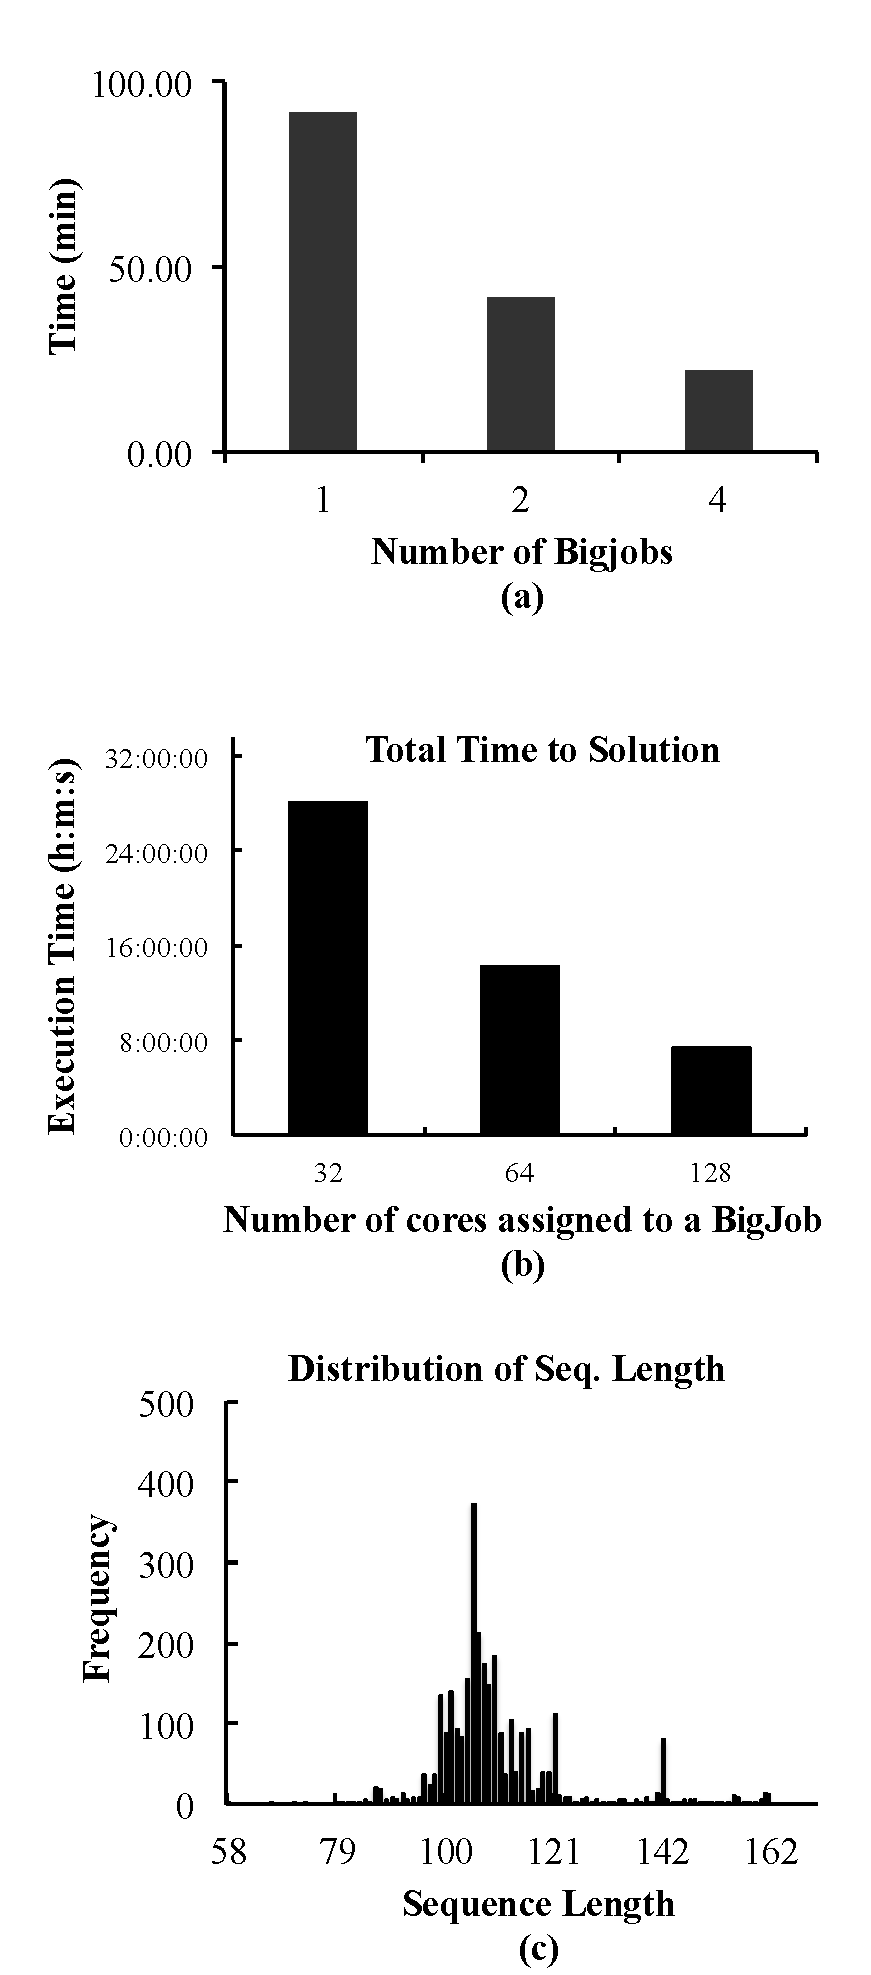
\includegraphics[scale=0.40]{figures/dare-rfold-result.pdf}
\caption{\small Massive concurrent calculation capability is presented with the results obtained with DARE-RFOLD. The total 2910 SAM-I riboswitch sequences are injected into the DARE-RFOLD for sampling of Boltzman-weighted secondary structures.  SAGA-BigJob handles these many tasks by decoupling the resource assignment and execution of each task, collectively allowing an efficient management of many tasks. In (a) and (b), time-to-solutions with different configurations of BigJob are compared in terms of the number of BigJobs (a) and the size of a BigJob (b).  In (c), the distribution of sizes of 2910 input sequences is illustrated.  This distribution is directly associated with the distribution of time-to-solutions of all 2910 tasks. The data are taken from the recent work\cite{ccpe11}.}
  \label{fig:dare-rfold-result} 
\end{figure}

Recently, we reported our exploration of NGS analytics using DARE-NGS
with the HPC grid such as TeraGrid and Cloud environment of
FutureGrid\cite{ecmls11}.  Using the results obtained from such an
effort, we present the comparison of various execution scenarios with
multiple resources including a cloud system in
Table~\ref{table:NGS-Distributed}.  While this demonstrates the
capability of DARE-NGS for utilizing HPC grids and a cloud environment
together or separately, our initial results, also, indicated several
issues with an emerging distributed environment.  For example, we
observed that the large data management in FutureGrid cloud demanded
to use Walrus data storage system, but an access by multiple VM's
failed often.  This kind of situations should be managed appropriately
since our case with human genome mapping requires disk space more than
the default disk space of the current cloud
environment. Interestingly, we could come up with a solution to
resolve such disk space issue by implementing different task level
concurrency, but it is apparent that a gateway development should be
flexible and agile for future changes in resources and computing
environments.

 \begin{table}
 \small
 \begin{tabular}{|c|c|c|c|c|c|c|c|c|} 
 \hline 
	                      &  Index File	&Raw &	Processed\\
	                      &&Short Reads& Short Reads\\
\hline 
Size  (GB)    	             &127&	9	&3.81\\
 \hline                       
LW to QB (s)   & 1814.29&	128.57&  -\\
  \hline
LW to Ranger(s) & 21166.67 & - & -\\
   \hline
LW to QB(s)    & 7105.67& - &-\\
 \& QB to Ranger(s)     &&&\\
 \hline
QB to Ranger(s)   	&-&-& 158.33\\
\hline
Min Total time(s)    &	7105 &	128&	158.33\\
 \hline
\end{tabular}
\caption{File transfer time with GridFTP between a local workstation (LW), QueenBee (QB), and Ranger with the case of Human Genome index files and exome data.  }

 \label{table:NGS-Distributed-file} 
\end{table}

As sated before, for the data-intensive computation such as NGS
analytics, file transfer processes are important for the total
time-to-completion, and Table~\ref{table:NGS-Distributed-file} hints
such issues with the measured transfer time obtained with DARE-NGS.
At this moment, our gateways employ GridFTP as a default protocol on
the grids such as Teragrid/LONI and SCP for FutureGrid Sierra Cloud.

\subsection{DARE-RFOLD}
To support nc-RNA research and broadly for the community who is
interested in the utilization of RNA structure prediction for their
research goals and education purposes, we have been developing a
gateway, DARE-RFOLD, with which a user is able to predict the Minimum
Free Energy (MFE) secondary structure or an ensemble of structure
sampled with a Boltzmann-weighted sampling scheme.

Notably, our investigation on the computational requirements of RNA
folding dynamics suggested that the support of high-throughput
computation for a large number of tasks on heterogeneous distributed
resources is beneficial for the exploration of RNA folding energy
landscape and structural characterization of SAM-I riboswitch
sequences.  As shown in Fig.~\ref{fig:dare-rfold-result}, with the
DARE framework and its capacity for implementing a many-task-computing
support, we could carry out the total 2910 tasks needed for all
well-known SAM-I RAN family with different configurations for BigJob
set up\cite{ecmls10}.


\subsection{DARE-DOCK}
DARE-DOCK was developed to support the basic virtual screening and for
the current implementation, the gateway supports the docking with a
popular application, Autodock\cite{autodock}.  Recently announced
Autodock-vina is used as a main tool since the application further
supports fine-grain parallelism with multi-threading multi-core
support, whose new capabilities are thus considerably suitable for a
multiple resource execution since a simple pre-proccesing on a target
chemical database allows to implement virtual screening on
heterogeneous distributed resources\cite{autodock-vina}.

%\begin{figure}
% \centering
%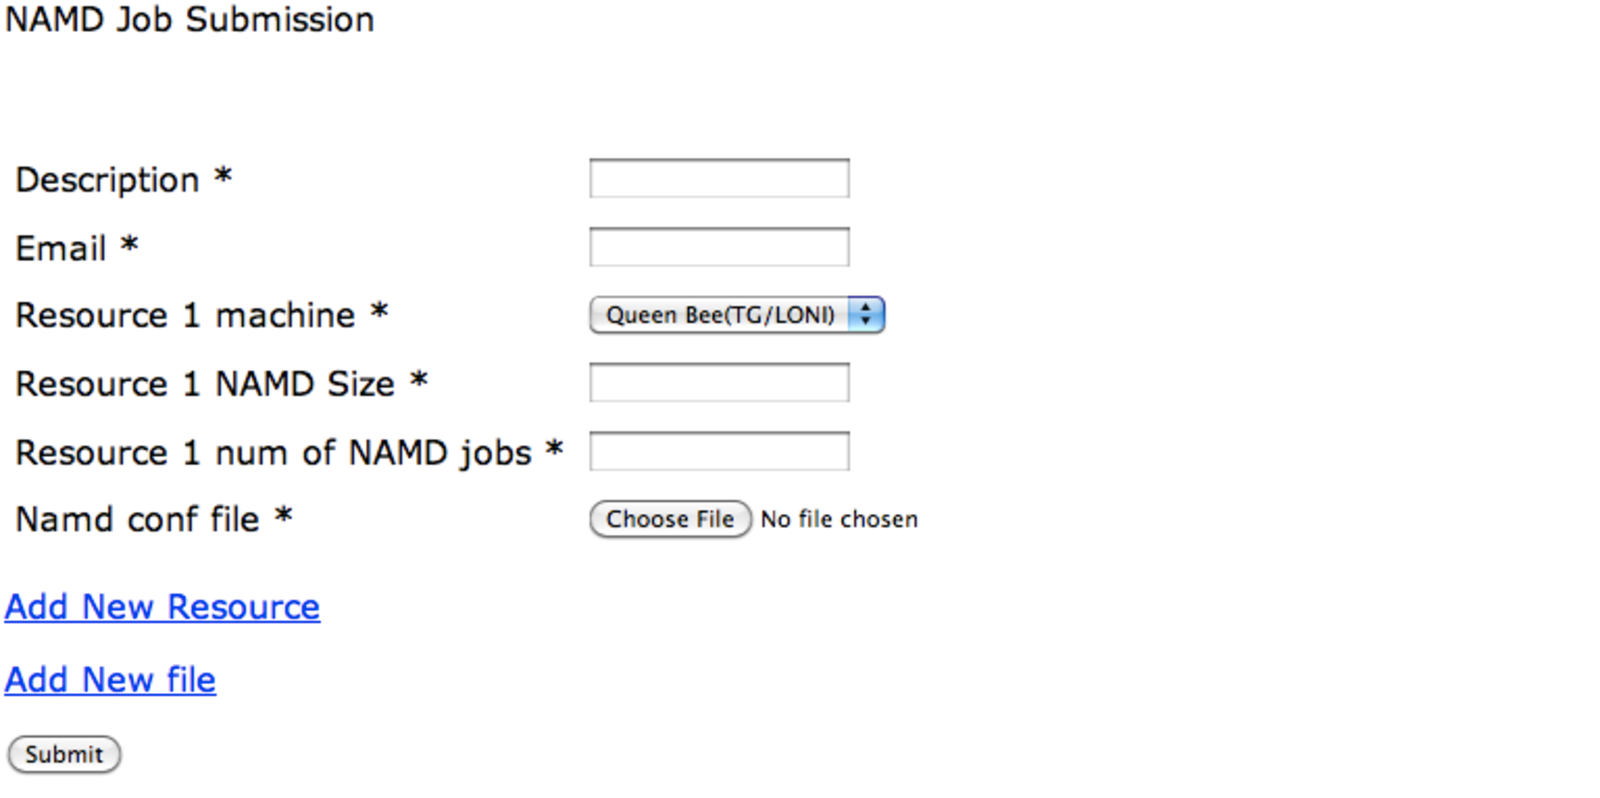
\includegraphics[scale=0.35]{figures/NAMD1.pdf}
%
%\caption{\small NAMD job submission web page form through DARE-HTHP} 
%\end{figure}

\subsection{DARE-HTHP}

An important challenge in modern biomolecular simulations, that has
received insufficient attention is not to get single long-running job
completed, but managing and executing multiple instances of the same
(or similar) physical system.  There are multiple reasons behind this
-- ranging from higher accuracy to reduced time-to-solution. For
example, multiple ensemble-member runs of the same physical system
enable better sampling In some cases, such as free-energy
calculations, multiple ensembles of the same system need to be
utilized. And even where a single long-running simulation is required,
thanks to algorithmic advances, such problems can be transformed into
the more {\it tractable} problem of solving multiple shorter run
simulations.



An ensemble simulation framework is required which has the following
characteristics: (i) Usable on a range of underlying distributed
resources and independent of the machine/resource-specific middleware
and services (i.e. scale-across), (ii) Efficiently manage both
scale-up and scale-out of ensembles -- possibly scaling upto
tens-of-thousands, if not millions of ensembles, with varying degrees
of coupling, (iii) Effective for a range of physical model sizes --
from thousands of atoms to hundreds of thousands of atoms, (iv) All of
the above without being tied to a specific underlying MD kernel, (v)
Extensible and Interoperable with emerging computational platforms
such as clouds.  Our results presented in
Table~\ref{table:HTHP-Distributed} clearly show that the DARE-HTHP is
able to run such an ensemble simulations.

\jkimnote{need the attention for the following. one or two sentence
  summary would be desirable}

%When the user submits the job to run on Futuregrid cloud environment
%the input files are transferred to different VM's. The configuration
%files that are prepared in the Access/Application layer will be used
%to launch the DARE Framework which in turn starts/submits according
%to the job configuration provided by user across Grids and Clouds.

To provide the capability to run jobs in cloud using DARE, we have
prepared images which have SAGA and other required adaptors installed
along with NAMD and MPI as well.  These images are used to launch
multiple VM's and job submission similar to grid environment. Further
we are in a process of proving a capabilty where a user can upload
their images, and DARE will transfer them to Eucalyptus cloud on
Futuregrid and run on virtualized environment; it is also responsible
for marshalling the VM's and tasks in these environments.

 \begin{table}
\small
 \begin{tabular}{|c|c|c|c|c|c|c|} 
 \hline 
 Number           & Resource    & \# of &  \# of     &     \# of     &	TTC  \\
of tasks                &     &  Cores    &nodes&   VMs  & (sec) \\  
\hline
8& R&	64	&4 & - &141\\
\hline                  
8& QB	&	64& 8 &	-&176 \\
\hline
4/4&R/QB	&	32/32 &2/4&-&151\\
\hline
8&FG	&	64(8) & - &8&414 \\
\hline
2/3/3&R/QB/FG	&32/24/24&2/3&	3 &384\\
\hline


\end{tabular}
\caption{8 tasks of NAMD run over different resources, Three compute resources are Ranger (R), QueenBee (QB), and  FutureGrid  Eucalyptus Cloud on Sierra(FG), respectively.}

  \label{table:HTHP-Distributed} 
\end{table}


\begin{figure}
 \centering
 \fbox{

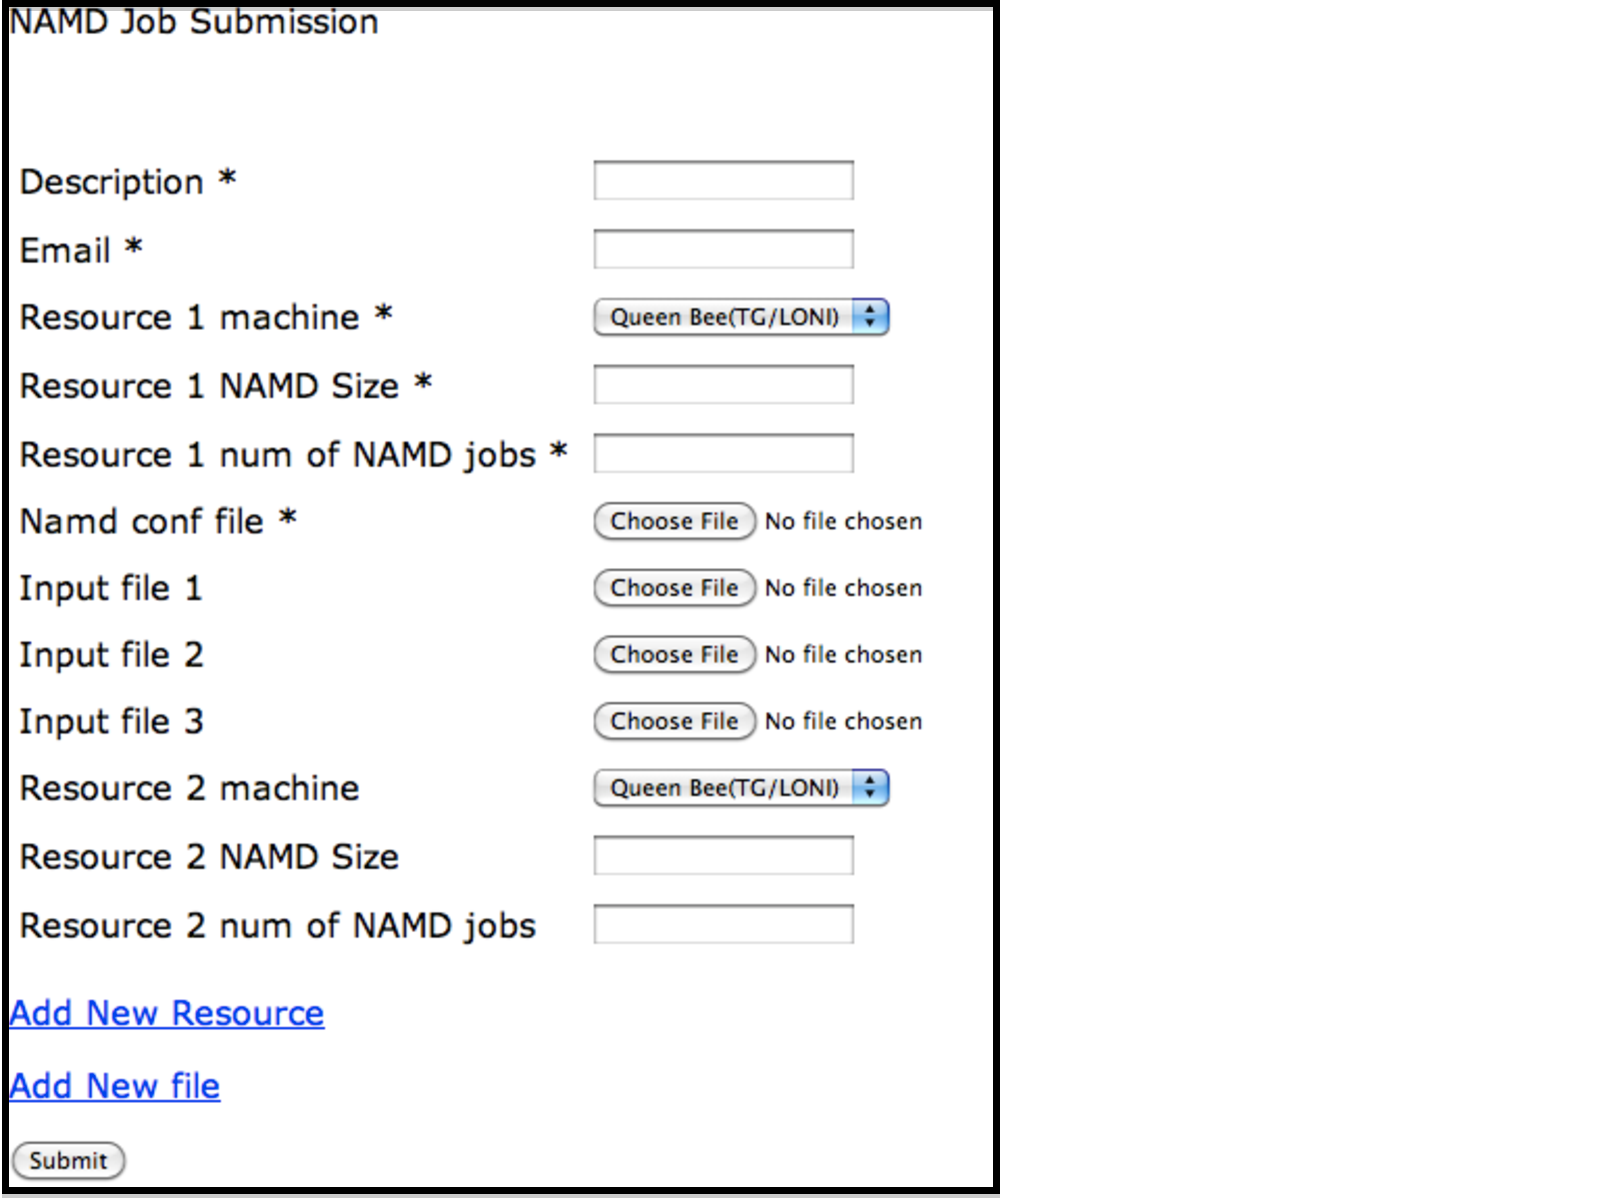
\includegraphics[scale=0.35]{figures/NAMD2.pdf}
   
  }
\caption{\small NAMD job submission web page form through
  DARE-HTHP. Here, the form indicates the usage mode with multiple
  resources.  The simple case with a single resource is default, and a
  user can expands the form by adding more resources as shown.
  DARE-HTHP can be accessed at:
  \url{http://cyder.cct.lsu.edu/dare-hthp} }
  \label{fig:NAMD2}
\end{figure}


\section{Conclusions}

% \textit{Achieving IDEAS : Interoperability, Distributed
%   scaled-out, Extensibility, Adaptivity, and Simplicity}

%\smnote{ 1) Lets say we have "n" read files and with DARE it takes
%  around time "t" time for matching step if we run it serially it
%  would take n*t time. It probably exceeds wall time limit. Therefore
%  speed up in match step depends how many number of read files we
%  generate and process concurrently.  2) Yes we were able to process
%  the complete run with entire Human Genome on QB and Ranger
%  separately. (**I am currently working this to utilizing QB and
%  Ranger together.)  4) it should clearly provide the advantage with
%  multiple resources. If we want to use the cloud resources from India
%  to complete Human Genome run it is not practically possible because
%  of the current limited disk size access provided by the FG
%  Eucalyptus resources. Because whole human genome index files are of
%  size 129 GB for Bfast matching step as opposed to HG 18 Chromosome
%  21 with size of 2 GB index files. On the other hand it also requires
%  the temporary files disk space.  Thus it is important to utilize
%  large capacity resources like QB and Ranger divide the work load
%  across machines.}  
  
%   Here, we present how the objectives of IDEAS\cite{ideas} are
% accomplished with the DARE gateway examples. 

All of components in the DARE framework are independent to each other
due to its modular structure.  Additionally, the framework provides
the key functionality for job management and data management with
heterogeneous distributed resources in a flexible mechanism to support
various execution patterns and application usage modes as well as the
full-fledge access layer with the web server framework.  Along with
this backbone template, a developer can quickly implement his/her own
scientific logic in the application layer with python scripts.

The objective {\it Distributed scale-out} is illustrated in with
Table~\ref{table:NGS-Distributed}, where, two large TeraGrid systems,
QB and Ranger, were used for the match step in BFAST pipeline.  It is
noticeable that we compare different usage modes, for example, using
one resource or two resource altogether with the same configuration
for the computation.  As we demonstrated in numerous publications,
having more resources and using those scaled computing power benefits
to decrease the time-to-completion.  The results of the cases in
Table~\ref{table:NGS-Distributed} indicate also there are interesting
aspects due to the complexity of scientific applications.  For
example, in the NGS data alignment using BFAST, we should consider the
optimal condition with the task level concurrency considering how the
reference genome indexes are utilized for chucks of short read
data\cite{ecmls11}. Not only have we established efficient distributed
scale-out for data-intensive applications, we have shown the effective
distributed of multiple MD simulations -- both in loosely-coupled and
uncouped modes.

Extensibility is an important objective for DARE-based gateways, and
indeed, many levels of extensibility are easily provided and utilized.
While SAGA itself provides the capabilities to expand the
infrastructure it can be utilized on, via the adaptor mechanism, e.g.,
the SAGA-based approaches which provide numerous adaptors,
interoperability across different middleware types is limited only by
the availability of adaptors, as well as emerging new environment such
as clouds. SAGA and SAGA-BigJob, combined together, provides great
flexibility to extend scientific capability of a gateway, e.g.,
support of ensemble-based simulations as a primitive ``execution
unit''. With DARE-RFOLD, we made a pipeline for another capability
beyond RNA secondary structure prediction.  We demonstrated recently
that the output from the RNA secondary structure prediction could be
utilized for Riboswitch gene annotation with structural information.
Furthermore, with the open source pylons framework, incorporation of
web technologies is efficiently and easily achieved.

Adaptivity is provided h in the design of the DARE framework, as the
SAGA-based pilot-abstractions, support agile and dynamic execution
modes and the change of application usage modes (eg concurrent
multiple simulations to one large-scale simulation). In
Fig.~\ref{fig:dare-rfold-result}, the result compares two different
configurations of BigJob size.  Note that not only varying the size of
a BigJob, other possible usage modes supporting a case of loosely
coupled applications~\cite{coupled} and a case of dynamically changing
parallel/concurrent configurations in the fine-grain parallelization
(for example, MPI configuration) as well as the coarse-grain
parallelization are effectively designed.

Simplicity is provided by a well defined interface that supports
multiple {\it standards} distributed functionality, as well as
higher-level abstractions, e.g., based on the underlying SAGA-based
API, via SAGA-BigJob a general purpose Pilot-Job abstraction.

In summary, the DARE framework supports the IDEAS design-objectives of
distributed applications, and due to its easy integration with other
components, it enables the effective and easy development of science
gateway that supports distributed applications. This includes novel
data-intensive life-science applications that utilize emerging
distributed computing/data resources such as TeraGrid/XD and cloud
environment contributes.


\section{Acknowledgments}
We are grateful to Andre Luckow and Ole Weidner for their work for
SAGA and SAGA-BigJob development.  Computing resources used for this
work were made possible via NSF TRAC award TG-MCB090174 and LONI
resources.  This document was developed with support from the National
Science Foundation (NSF) under Grant No.  0910812 to Indiana
University for ``FutureGrid: An Experimental, High-Performance Grid
Test-bed.'' The project described was partially supported by Grant
Number P20RR016456 from the NIH National Center For Research
Resources. SJ would like to thank Dave Hart (SDSC) and Dan Katz
(Chicago) for helpful discussions.

\bibliographystyle{abbrv}
\bibliography{tg11}
\end{document}

